В ходе проведения компьютерной экспертизы может возникнуть необходимость 
проанализировать электронные письма злоумышлиника. Подобную информацию можно 
получить из файлов, сохраняемых программой OutLook на ПК пользователя. Для 
осуществления данной задачи был разработан программный модуль Outlook.

Почтовая программа (почтовый клиент, клиент электронной почты, мейлер, мейл-клиент) --- 
это ПО, которое инсталлируется на компьютер пользователя и предназначено для 
написания, получения, хранения, отправки электронной почты одного или нескольких 
пользователей (например, когда имеется несколько учетных записей на компьютере), или 
нескольких учетных записей пользователя.

Сообщения, синхронизированные с Outlook, имеют самой программе следующий вид (рис~\ref{ser_1:ser_1}). Задача 
модуля состоит из поиска данных, отображаемых в программе Outlook в бинарном файле <<.dbx>> (рис~\ref{ser_2:ser_2}). В результате работы модуля получаем списки всех тем, дат и тд. сообщения (рис~\ref{ser_3:ser_3}).

\begin{figure}[h!]
\center{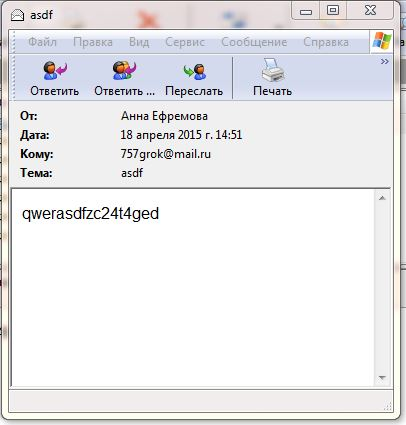
\includegraphics[width=0.6\linewidth]{ser_1}}
\caption{Сообщения, синхронизированные с Outlook}
\label{ser_1:ser_1}
\end{figure} 

\begin{figure}[h!]
\center{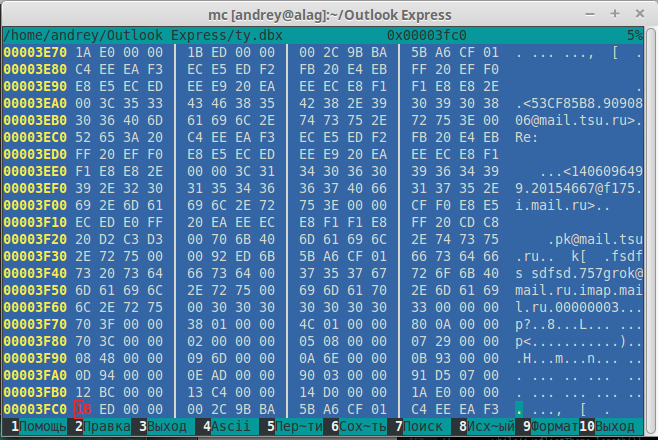
\includegraphics[width=0.8\linewidth]{ser_2}}
\caption{Содержание бинарного файла формата <<.dbx>>}
\label{ser_2:ser_2}
\end{figure} 

\begin{figure}[h!]
\center{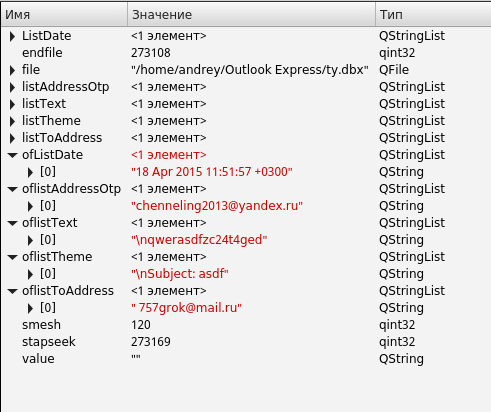
\includegraphics[width=0.8\linewidth]{ser_3}}
\caption{Результат работы модуля}
\label{ser_3:ser_3}
\end{figure} 

\clearpage
\subsubsection{Реализация программного модуля для почтового клиента MS Outlook}

Реализация данного программного модуля включала в себя следующие шаги:

\begin{enumerate}
  \item изучение бинарного формата данных <<.dbx>>;
  \item изучение регулярных выражений и библиотек для работы с ними в Qt C++;
  \item разработка поиска файлов формата <<.dbx>> на носителе, на котором установлен Outlook;
  \item разработка программы для считывания не всего файла, а только его части, чтобы тем самым 
  уменьшить нагрузку на оперативную память;
  \item разработка регулярных выражений для поиска адресата, отправителя, темы, даты и 
  текста сообщения и создание парсера для части информации, извлекаемой из файла;
  \item изучение особенностей работы с XML-форматом (языком разметки) и разработка класса для 
  записи данных, полученных из парсера, в XML;
  \item изучение системы распределенного контроля версий Git и ее основных возможностей;
  \item изучение различных файловых форматов, таких как PST, PAB, MSG, RTF, HTML.  
\end{enumerate}

Трудности, возникшие при написании модуля:

\begin{enumerate}
  \item В начале написания модуля  возникла явная проблема переполнения оперативной 
  памяти из-за добавления всего файла целиком в поток главной программы. 
  Появилась потребность в написании программы, которая делила бы файл на части, 
  запоминала место конца предыдущей части программы и начинала отделять часть 
  такой же длины. Кроме того, данная программа должна была считывать часть файла из любого его места, 
  которую укажут в параметрах, а также преобразовывать последовательность бит в строку юникода. 
  После чего была разработана и написана программа, реализующая данную потребность.
  \item Далее стала необходимой разработка парсера (некоего фильтра данных), который бы находил и 
  забирал из выбранной части файла нужные нам последовательности бит. Были изучены основы регулярных 
  выражений, а также синтаксис составления шаблонов для класса QTRegex, реализующего работу с  
  регулярными выражениями в QT C++, включая сам класс QTRegex. Блок-схема данного парсера представлена 
  на рисунке~\ref{ser_4:ser_4}.
  \item Далее необходимо было разработать алгоритм занесения полученных данных в какой-либо 
  файл для их хранения. В связи с тем, что проект <<coex>> использует для вывода данных 
  файлы формата XML, был изучен данный формат, а также классы для работы с ним в QT C++. 
  После чего был написан класс <<WriteAddress>>, осуществляющий запись данных из парсера в XML. 
\end{enumerate}

Блок-схема исходного модуля после всех преобразований и дополнений приняла следующий вид
(рис.~\ref{ser_5:ser_5}).

\begin{figure}[h!]
\center{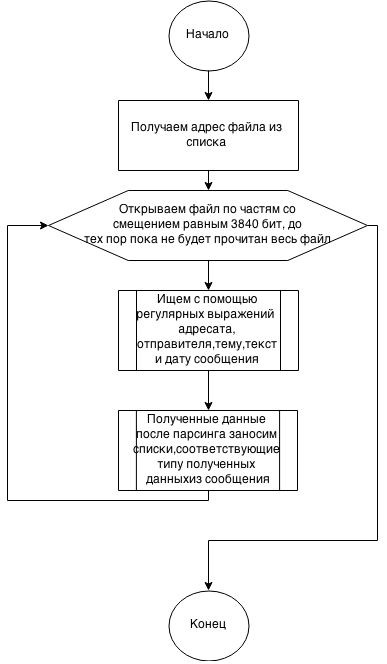
\includegraphics[width=0.6\linewidth]{ser_4}}
\caption{Блок-схема парсера для работы с битовыми строками}
\label{ser_4:ser_4}
\end{figure} 

\begin{figure}[h!]
\center{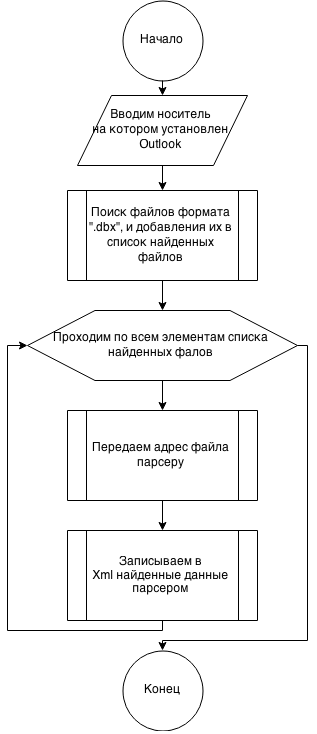
\includegraphics[width=0.5\linewidth]{ser_5}}
\caption{Блок-схема исходного модуля Outlook}
\label{ser_5:ser_5}
\end{figure} 

\subsubsection{Задачи на следующий семестр}

В следующем семестре планируется переделать поиск фалов не только в стандартном 
расположении (месте установки) Outlook, но и в других директориях, за непродолжительное 
время. Также планируется увеличить скорость работы модуля путем распараллеливания  потоков.

\clearpage
